\documentclass{standalone}
\usepackage{tikz}
\usetikzlibrary{decorations.markings}
\usetikzlibrary{arrows.meta}
\tikzset{% style to add an arrow in the middle of a path
  mid arrow/.style={postaction={decorate,decoration={
        markings,
        mark=at position .5 with {\arrow[#1]{Stealth}}}}}}
\makeatletter
\newcommand*\intToChar[1]{\@Alph{#1}}
\makeatother
\begin{document}

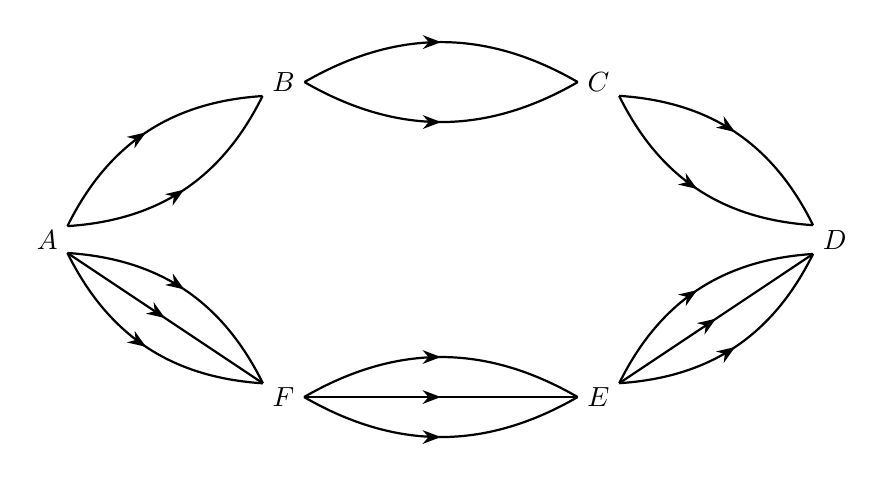
\begin{tikzpicture}
% Axes
%\draw[help lines, color=gray!30, dashed] (-7, -7) grid (7, 7);
%\draw[->,ultra thick] (-7,0)--(7,0) node[right]{$x$};
%\draw[->,ultra thick] (0, -7)--(0, 7) node[above]{$y$};

% First define nodes
\foreach[count=\cnt] \pnt/\lab in {(-5, 0)/A,
                                   (-2, 2)/B,
                                   ( 2, 2)/C,
                                   ( 5, 0)/D,
                                   ( 2,-2)/E,
                                   (-2,-2)/F}
  \node (\lab) at \pnt {$\lab$};
\path node also [alias=G] (A);

% Find points on their border to the other nodes
\foreach \lab[count=\cnt from 2] in {A, ..., F}
  \path (\lab) -- coordinate[at start] (\lab-to-\intToChar{\cnt})
                  coordinate[at end]   (\intToChar{\cnt}-to-\lab)
                  (\intToChar{\cnt});

% Draw the lines and curves
\path [thick, every edge/.append style={mid arrow}]
  foreach \A/\B in {A/B, B/C, C/D, G/F, F/E, E/D} {
   (\A-to-\B) edge [bend left] (\B-to-\A)
              edge [bend right] (\B-to-\A)
  }
  foreach \A/\B in {G/F, F/E, E/D} {
    (\A) edge (\B)
  }
  ;
\end{tikzpicture}
\end{document}